\section{Introduction to R}

\hidenum
\begin{frame}[noframenumbering]
\frametitle{Contents}
 \tableofcontents[currentsection,hideallsubsections]
\end{frame}
\shownum

\subsection{What is R?}

\begin{frame}
  \begin{block}{What is R?}\pause
  \begin{minipage}{.75\textwidth}
  \begin{itemize}[<+-|alert@+>]
    \item \emph{Lingua franca} for data analytics and statistical computing
    \item Part programming language, part data analysis
      package, syntax designed for data
  \end{itemize}
  \end{minipage}
  \hfill
  \begin{minipage}{.2\textwidth}
    \centering
\includegraphics[scale=.5]{../common/pics/logos/Rlogo_clear}
  \end{minipage}
  \begin{itemize}
    \item Dialect of S (Bell Labs, 1976)
    \item Licensed under GPL in 1995
    \item 2+ million users, dominates new work in Statistics
    \item Switzerland: highest per-capita use of R!
      {\tiny\tt http://blog.revolutionanalytics.com/2014/04/a-world-map-of-r-user-activity.html}
  \end{itemize}
\end{block}
\end{frame}


\begin{frame}
\vspace{-.1cm}
\begin{block}{Who uses R?}
\ \\[6.5cm]\ 
\end{block}
% top line
\Put(0,400){
\includegraphics[scale=1]{../common/pics/R_using_logos/oracle}}
\Put(222,400){
\includegraphics[scale=.12]{../common/pics/R_using_logos/kickstarter}}
\Put(115,400){
\includegraphics[scale=.1]{../common/pics/R_using_logos/merck}}
%%%%
% second line
\Put(-5,300){
\includegraphics[scale=.2]{../common/pics/R_using_logos/boa}}
\Put(87,300){
\includegraphics[scale=.2]{../common/pics/R_using_logos/fb}}
\Put(150,300){
\includegraphics[scale=.2]{../common/pics/R_using_logos/okcupid}}
\Put(218,320){
\includegraphics[scale=.35]{../common/pics/R_using_logos/nyt}}
%%%%
% third line
\Put(-16,180){
\includegraphics[scale=.05]{../common/pics/R_using_logos/shell}}
\Put(60,180){
\includegraphics[scale=.2]{../common/pics/R_using_logos/pfizer}}
\Put(155,180){
\includegraphics[scale=.9]{../common/pics/R_using_logos/mozilla}}
\Put(200,220){
\includegraphics[scale=.1]{../common/pics/R_using_logos/orbitz}}
\Put(204,160){
\includegraphics[scale=.16]{../common/pics/R_using_logos/lloyds}}
%%%%
% fourth line
\Put(-35,80){
\includegraphics[scale=.12]{../common/pics/R_using_logos/google}}
\Put(60,80){
\includegraphics[scale=.12]{../common/pics/R_using_logos/ebay}}
\Put(110,80){
\includegraphics[scale=.12]{../common/pics/R_using_logos/bing}}
\Put(170,80){
\includegraphics[scale=.29]{../common/pics/R_using_logos/ford}}
\end{frame}

\begin{frame}
  \begin{block}{Who integrates R?}
    \begin{minipage}[t]{4.5cm}
      \begin{itemize}
      \item SAS
      \item Tableau
      \item IBM-SPSS
      \item VTK (Paraview, VisIt)
      \item alteryx
      \end{itemize}
    \end{minipage}
    \begin{minipage}[t]{3cm}
      \begin{itemize}
      \item Omniscope
      \item Python
      \item Java
      \item ORACLE
      \item KNIME
      \end{itemize}
    \end{minipage}
    \begin{minipage}[t]{2.5cm}
      \begin{itemize}
      \item XCEL
      \item $\ldots$
      \end{itemize}
    \end{minipage}
  \end{block}
\end{frame}

\begin{frame}
  \begin{block}{Language Paradigms}\pause
  \begin{center}
    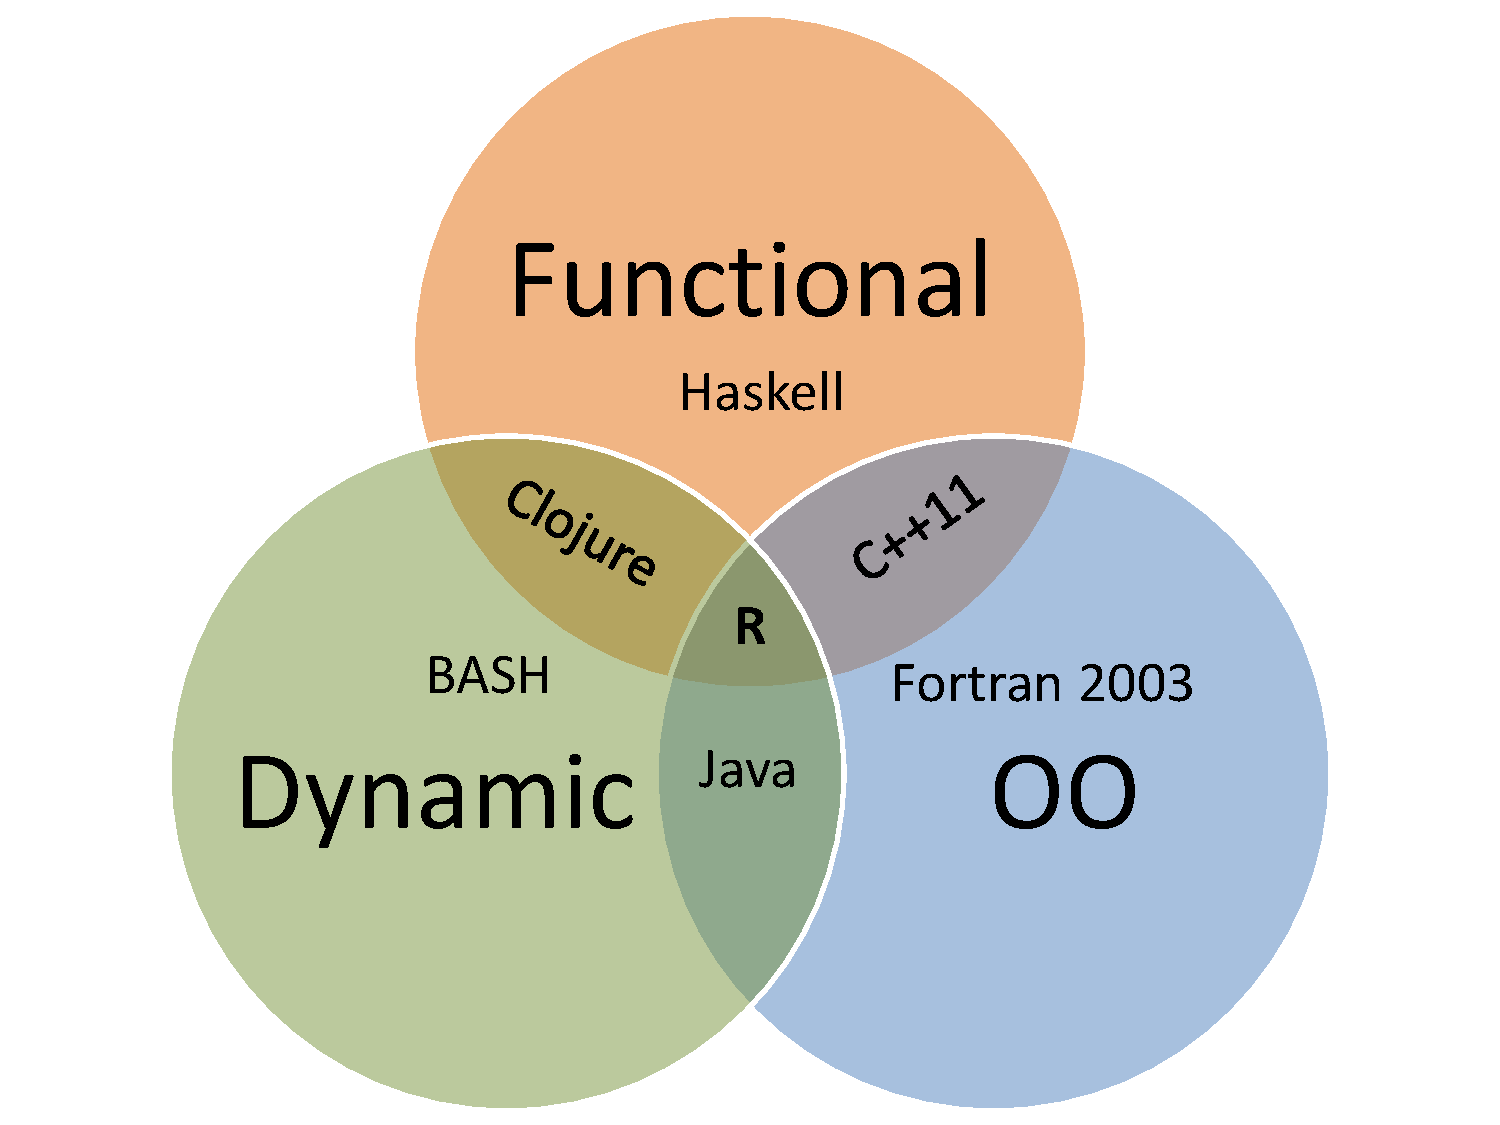
\includegraphics[scale=.35]{../common/pics/languages.pdf}
  \end{center}
  \end{block}
\end{frame}

\begin{frame}[fragile]
  \begin{block}{Dynamic Data Types}%\pause
    \begin{itemize}%[<+-|alert@+>]
    \item Storage:  logical, int, double, double complex, character
    \item Structures:  vector, matrix, array, list, dataframe
    \item Caveats:  (Logical) \code{TRUE}, \code{FALSE}, \code{NA}
    \end{itemize}
  \end{block}
  \begin{block}{High Level Syntax}%\pause
    \begin{lstlisting}
x <- matrix(rnorm(30), nrow=10)
x <- x[-1, 2:5]
xtx <- t(x) %*% x
xtx <- crossprod(x)
ans <- prcomp(log(abs(x) + 1))
ans <- glm(y ~ a + b + ns(u,12), binomial(), mydata)
plot(ans)
print(ans)
    \end{lstlisting}
  \end{block}
\end{frame}

\begin{frame}
  \begin{block}{CRAN Task View (5,000+ packages)
      {\tiny\tt http://cran.rstudio.com/web/views/}}
    \pause
    \scalebox{0.85}{\tiny
      \begin{tabular}{ll}
        Bayesian & Bayesian Inference \\
        ChemPhys & Chemometrics and Computational Physics \\
        ClinicalTrials &	Clinical Trial Design, Monitoring, and Analysis \\
        Cluster &	Cluster Analysis \& Finite Mixture Models \\
        DifferentialEquations &	Differential Equations \\
        Distributions &	Probability Distributions \\
        Econometrics &	Computational Econometrics \\
        Environmetrics &	Analysis of Ecological and Environmental Data \\
        ExperimentalDesign &	Design of Experiments (DoE) \& Analysis of Experimental Data \\
        Finance &	Empirical Finance \\
        Genetics &	Statistical Genetics \\
        Graphics &	Graphic Displays \& Dynamic Graphics \& Graphic Devices \& Visualization \\
        HighPerformanceComputing &	High-Performance and Parallel Computing with R \\
        MachineLearning & Machine Learning \& Statistical Learning \\
        MedicalImaging &	Medical Image Analysis \\
        MetaAnalysis &	Meta-Analysis \\
        Multivariate &	Multivariate Statistics \\
        NaturalLanguageProcessing &	Natural Language Processing \\
        NumericalMathematics &	Numerical Mathematics \\
        OfficialStatistics &	Official Statistics \& Survey Methodology \\
        Optimization &	Optimization and Mathematical Programming \\
        Pharmacokinetics &	Analysis of Pharmacokinetic Data \\
        Phylogenetics &	Phylogenetics, Especially Comparative Methods \\
        Psychometrics &	Psychometric Models and Methods \\
        ReproducibleResearch &	Reproducible Research \\
        Robust &	Robust Statistical Methods \\
        SocialSciences &	Statistics for the Social Sciences \\
        Spatial &	Analysis of Spatial Data \\
        SpatioTemporal &	Handling and Analyzing Spatio-Temporal Data \\
        Survival &	Survival Analysis \\
        TimeSeries &	Time Series Analysis \\
        WebTechnologies &	Web Technologies and Services \\
        gR & gRaphical Models in R
      \end{tabular}}
  \end{block}
\end{frame}
% "The main difficulty is finding what you want, and understanding
% what you find" Eric Feigelson, Center for Astrostatistics, Penn State
\begin{frame}
  \begin{block}{Other R pakage repositories}
    \begin{itemize}
    \item 
\includegraphics[width=.2\textwidth]{../common/pics/logos/logo_bioconductor.jpg}
      \pause
      \begin{itemize}
      \item Tools for the analysis and comprehension of high-throughput
        genomic data
      \item 800+ packages {\tt http://www.bioconductor.org}
      \end{itemize}
    \item Rmetrics
      \begin{itemize}
      \item 30+ packages for financial computing {\tt https://rmetrics.org} (ETH)
      \end{itemize}
    \item $\ldots$
    \end{itemize}
  \end{block}
\end{frame}


\subsection{R and HPC}


\begin{frame}
  \begin{block}{Why take R to HPC?}
    \pause
    \begin{enumerate}[<+-|alert@+>]
      \item People love it
      \item Highly extensible
      \item Unmatched diversity of analytical methods
      \item Thorough treatment of uncertainty throughout
      \item Gold standard for graphics (traditional, grid, and ggplot2)
      \item HPC community needs a high-level language for data analysis
    \end{enumerate}
  \end{block}
\end{frame}

\begin{frame}
  \begin{block}{Data analysis is interactive!}
    \pause
    \begin{itemize}[<+-|alert@+>]
    \item Data reduction to knowledge
    \item S (and R) interactive ``answer'' to batch data analysis
    \item Efficient use of expensive people
    \item Iterative process with same data
      \begin{itemize}
      \item Diagnostics of fit
      \item Quantification of uncertainty
      \item Interpretation of results
      \end{itemize}
    \end{itemize}
  \end{block}
  \begin{block}{HPC is batch!}
    \pause
    \begin{itemize}[<+-|alert@+>]
    \item Traditionally data generation
    \item Efficient use of expensive platforms
    \item Long time to assimilate generated data
    \end{itemize}
  \end{block}
\end{frame}


\begin{frame}
\begin{block}{\scriptsize R Interfaces to Native Tools}
    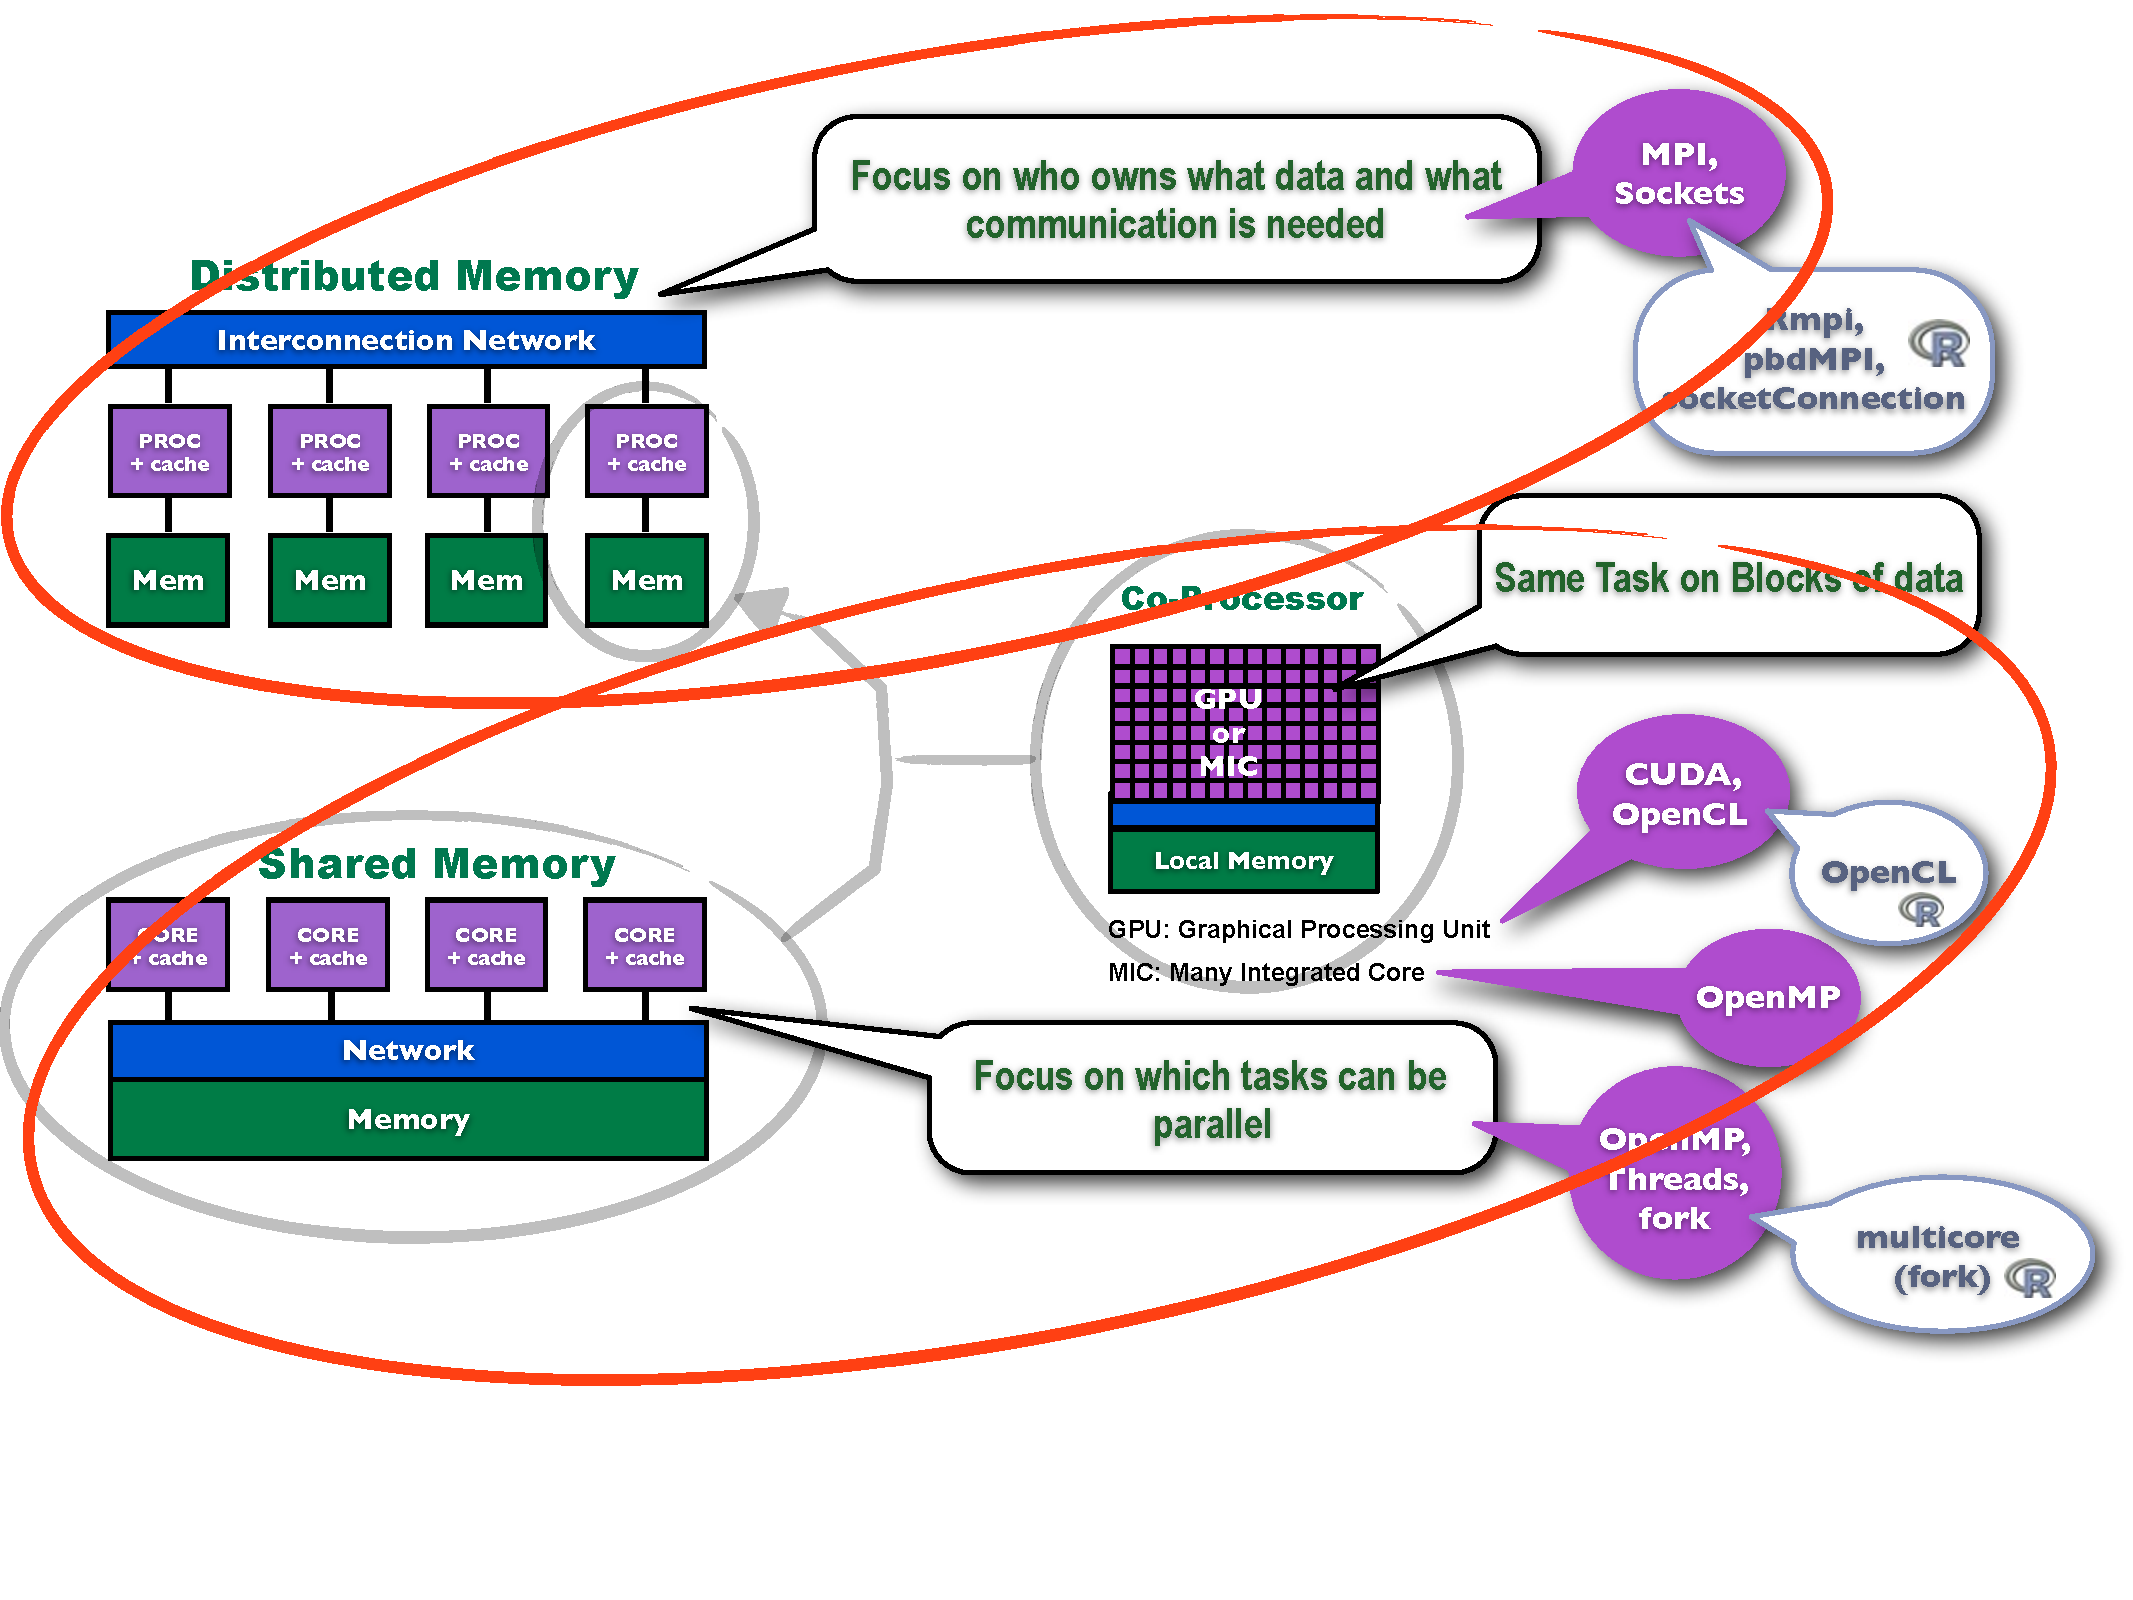
\includegraphics[width=\textwidth,trim=0ex 20ex 0ex 0ex,clip]{../common/pics/hardware/ParallelHardware10.pdf}
  \end{block}
\end{frame}

\begin{frame}
  \begin{block}{\scriptsize Scalable Math Libraries from 30+ Years of Research}
    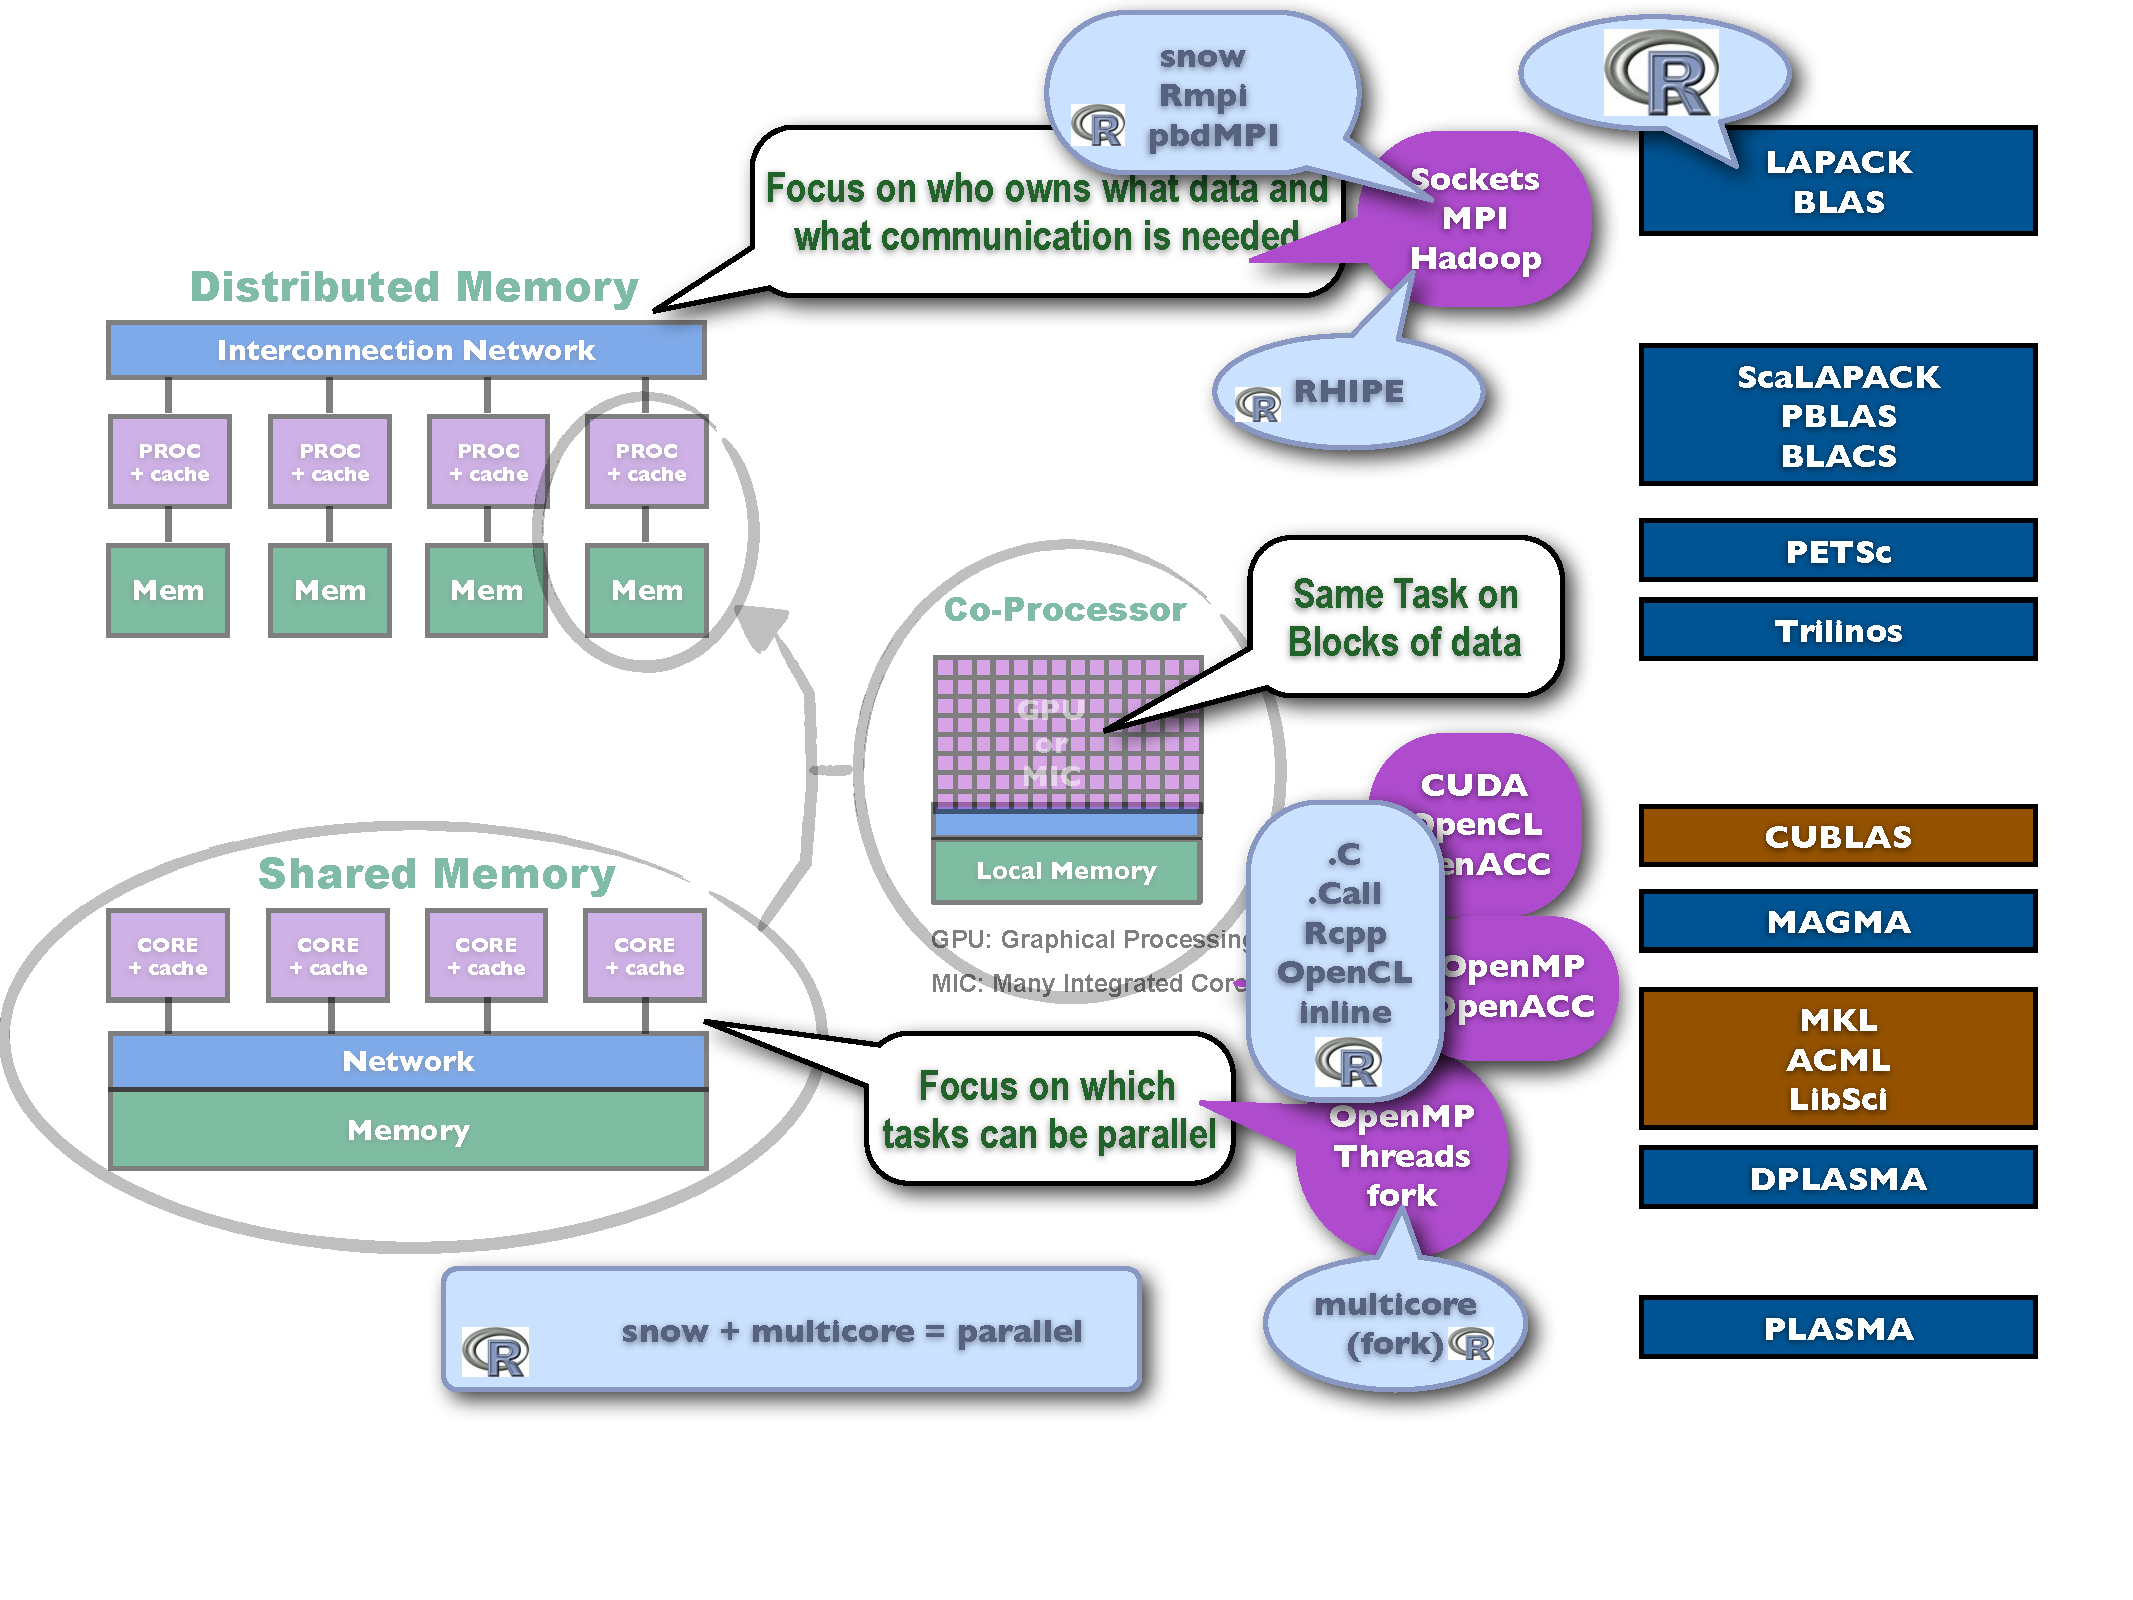
\includegraphics[width=\textwidth,trim=0ex 20ex 0ex 0ex,clip]{../common/pics/hardware/ParallelHardware11.pdf}
  \end{block}
\end{frame}

\begin{frame}
  \begin{block}{\scriptsize R Interfaces to Scalable Math Libraries}
    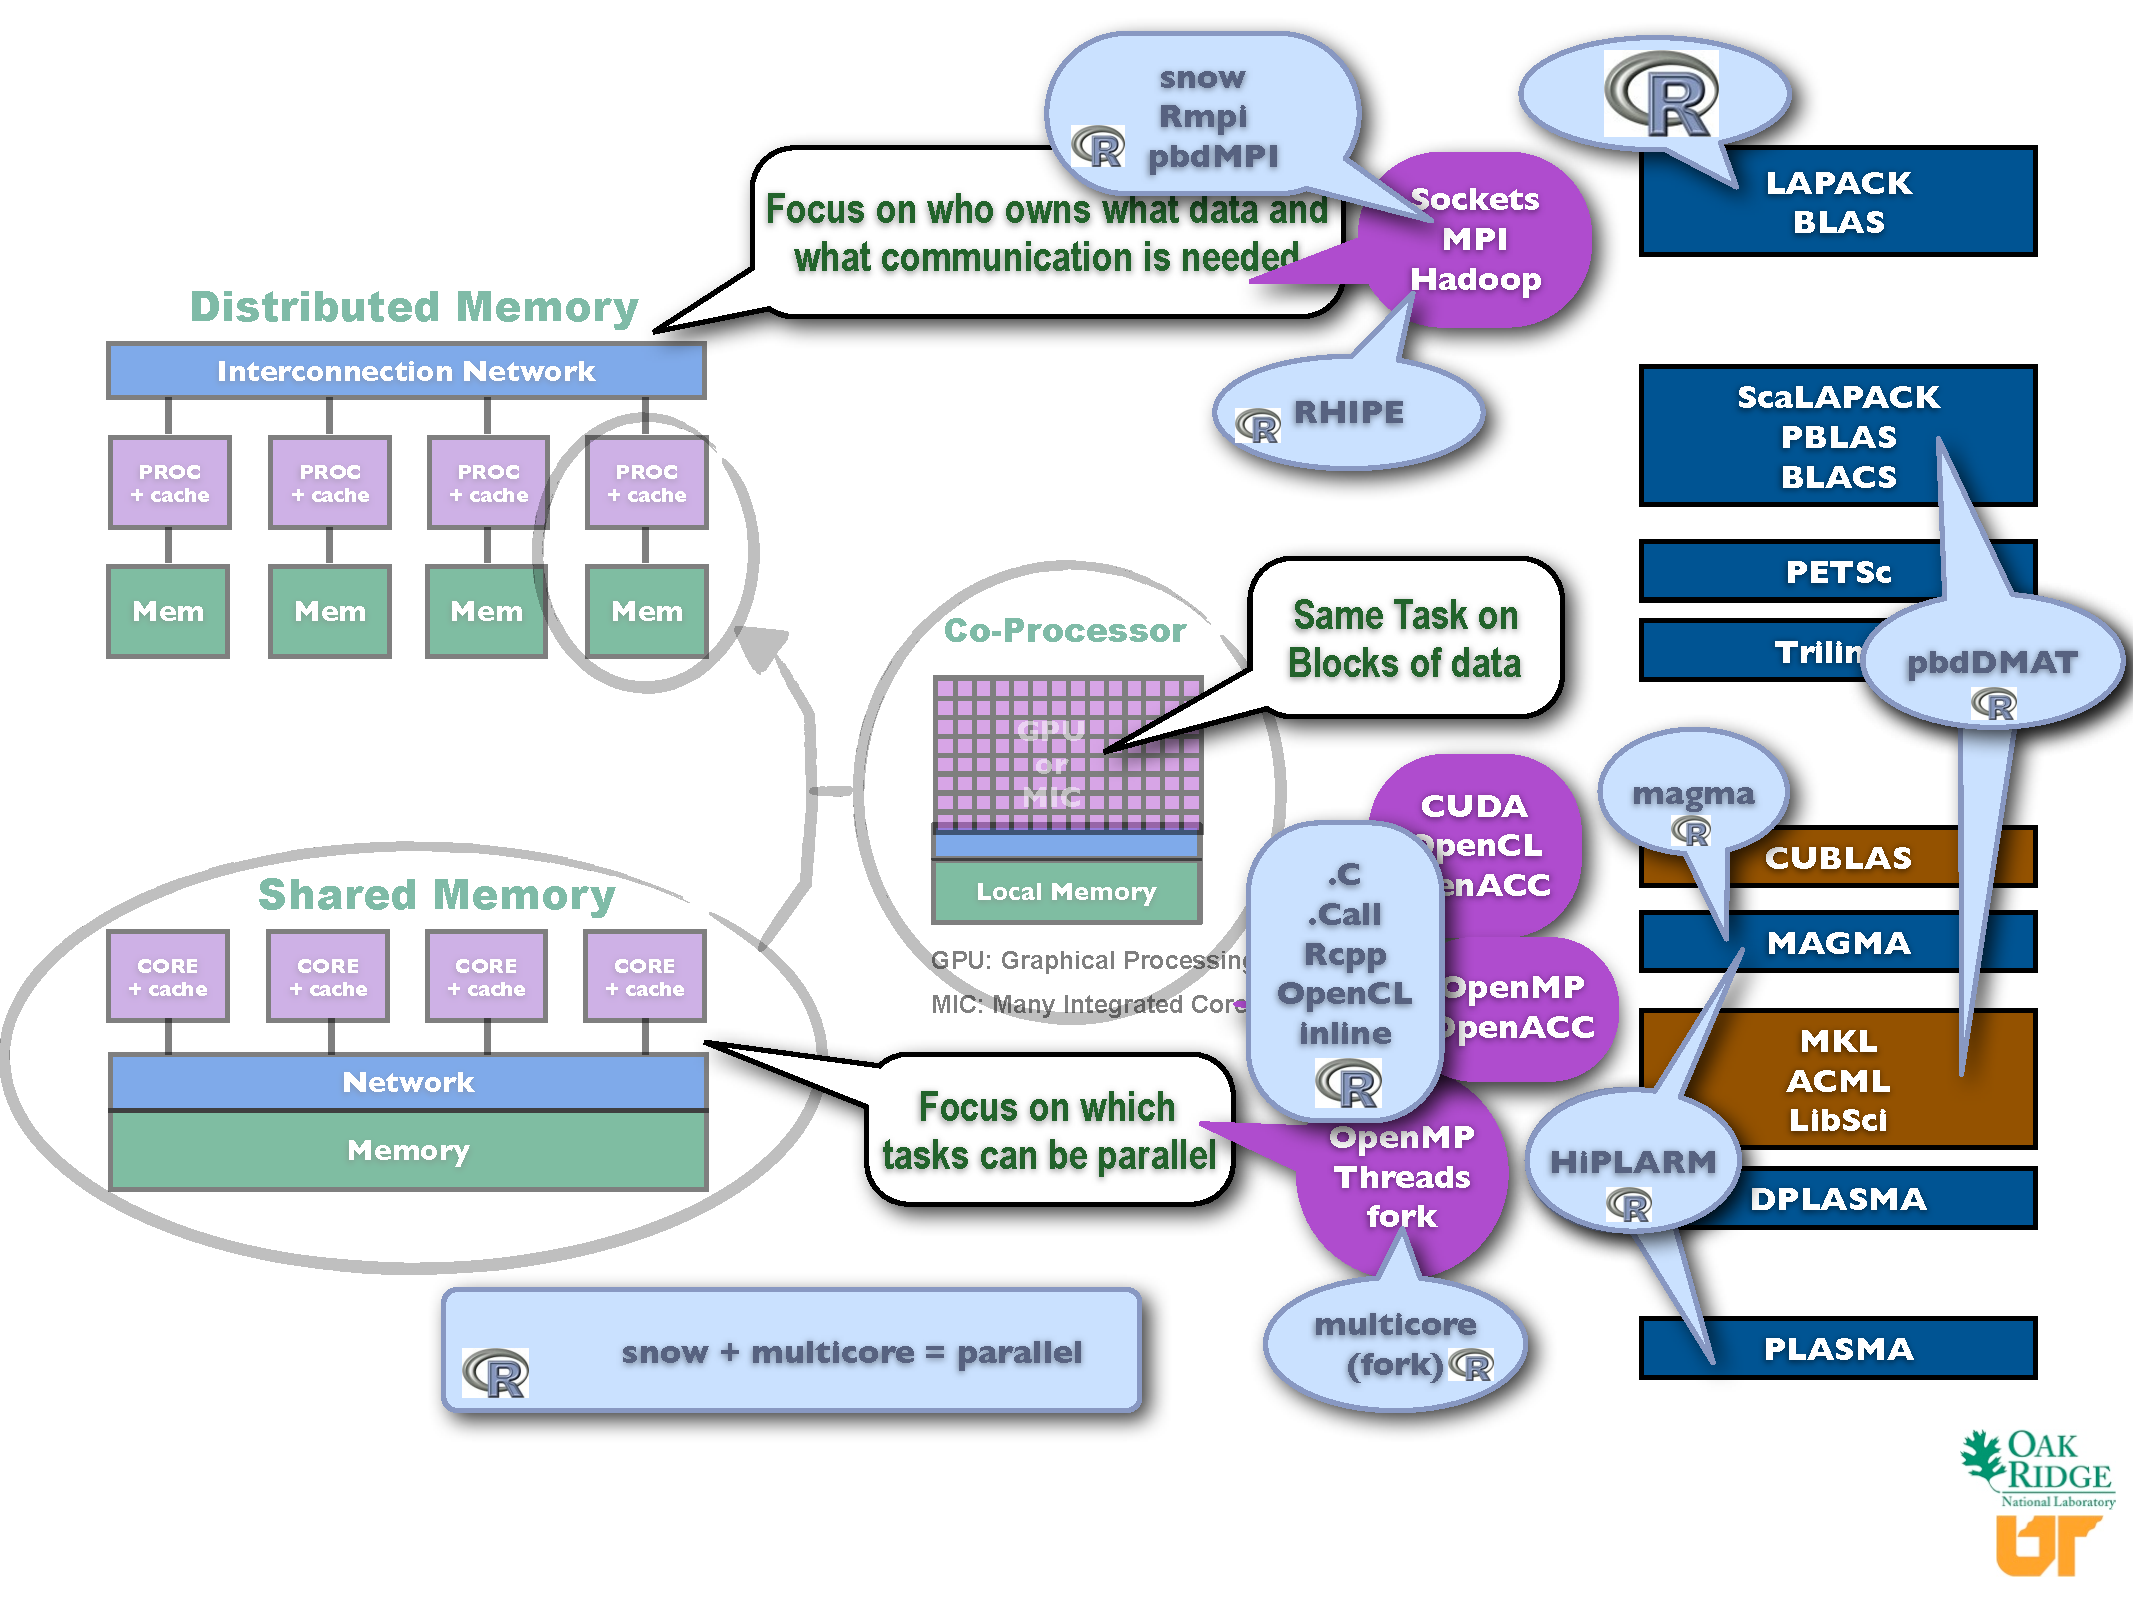
\includegraphics[width=\textwidth,trim=0ex 20ex 0ex 0ex,clip]{../common/pics/hardware/ParallelHardware12.pdf}
  \end{block}
\end{frame}
 
\begin{frame}
  \begin{block}{\scriptsize R Interfaces to Scalable Math Libraries}
    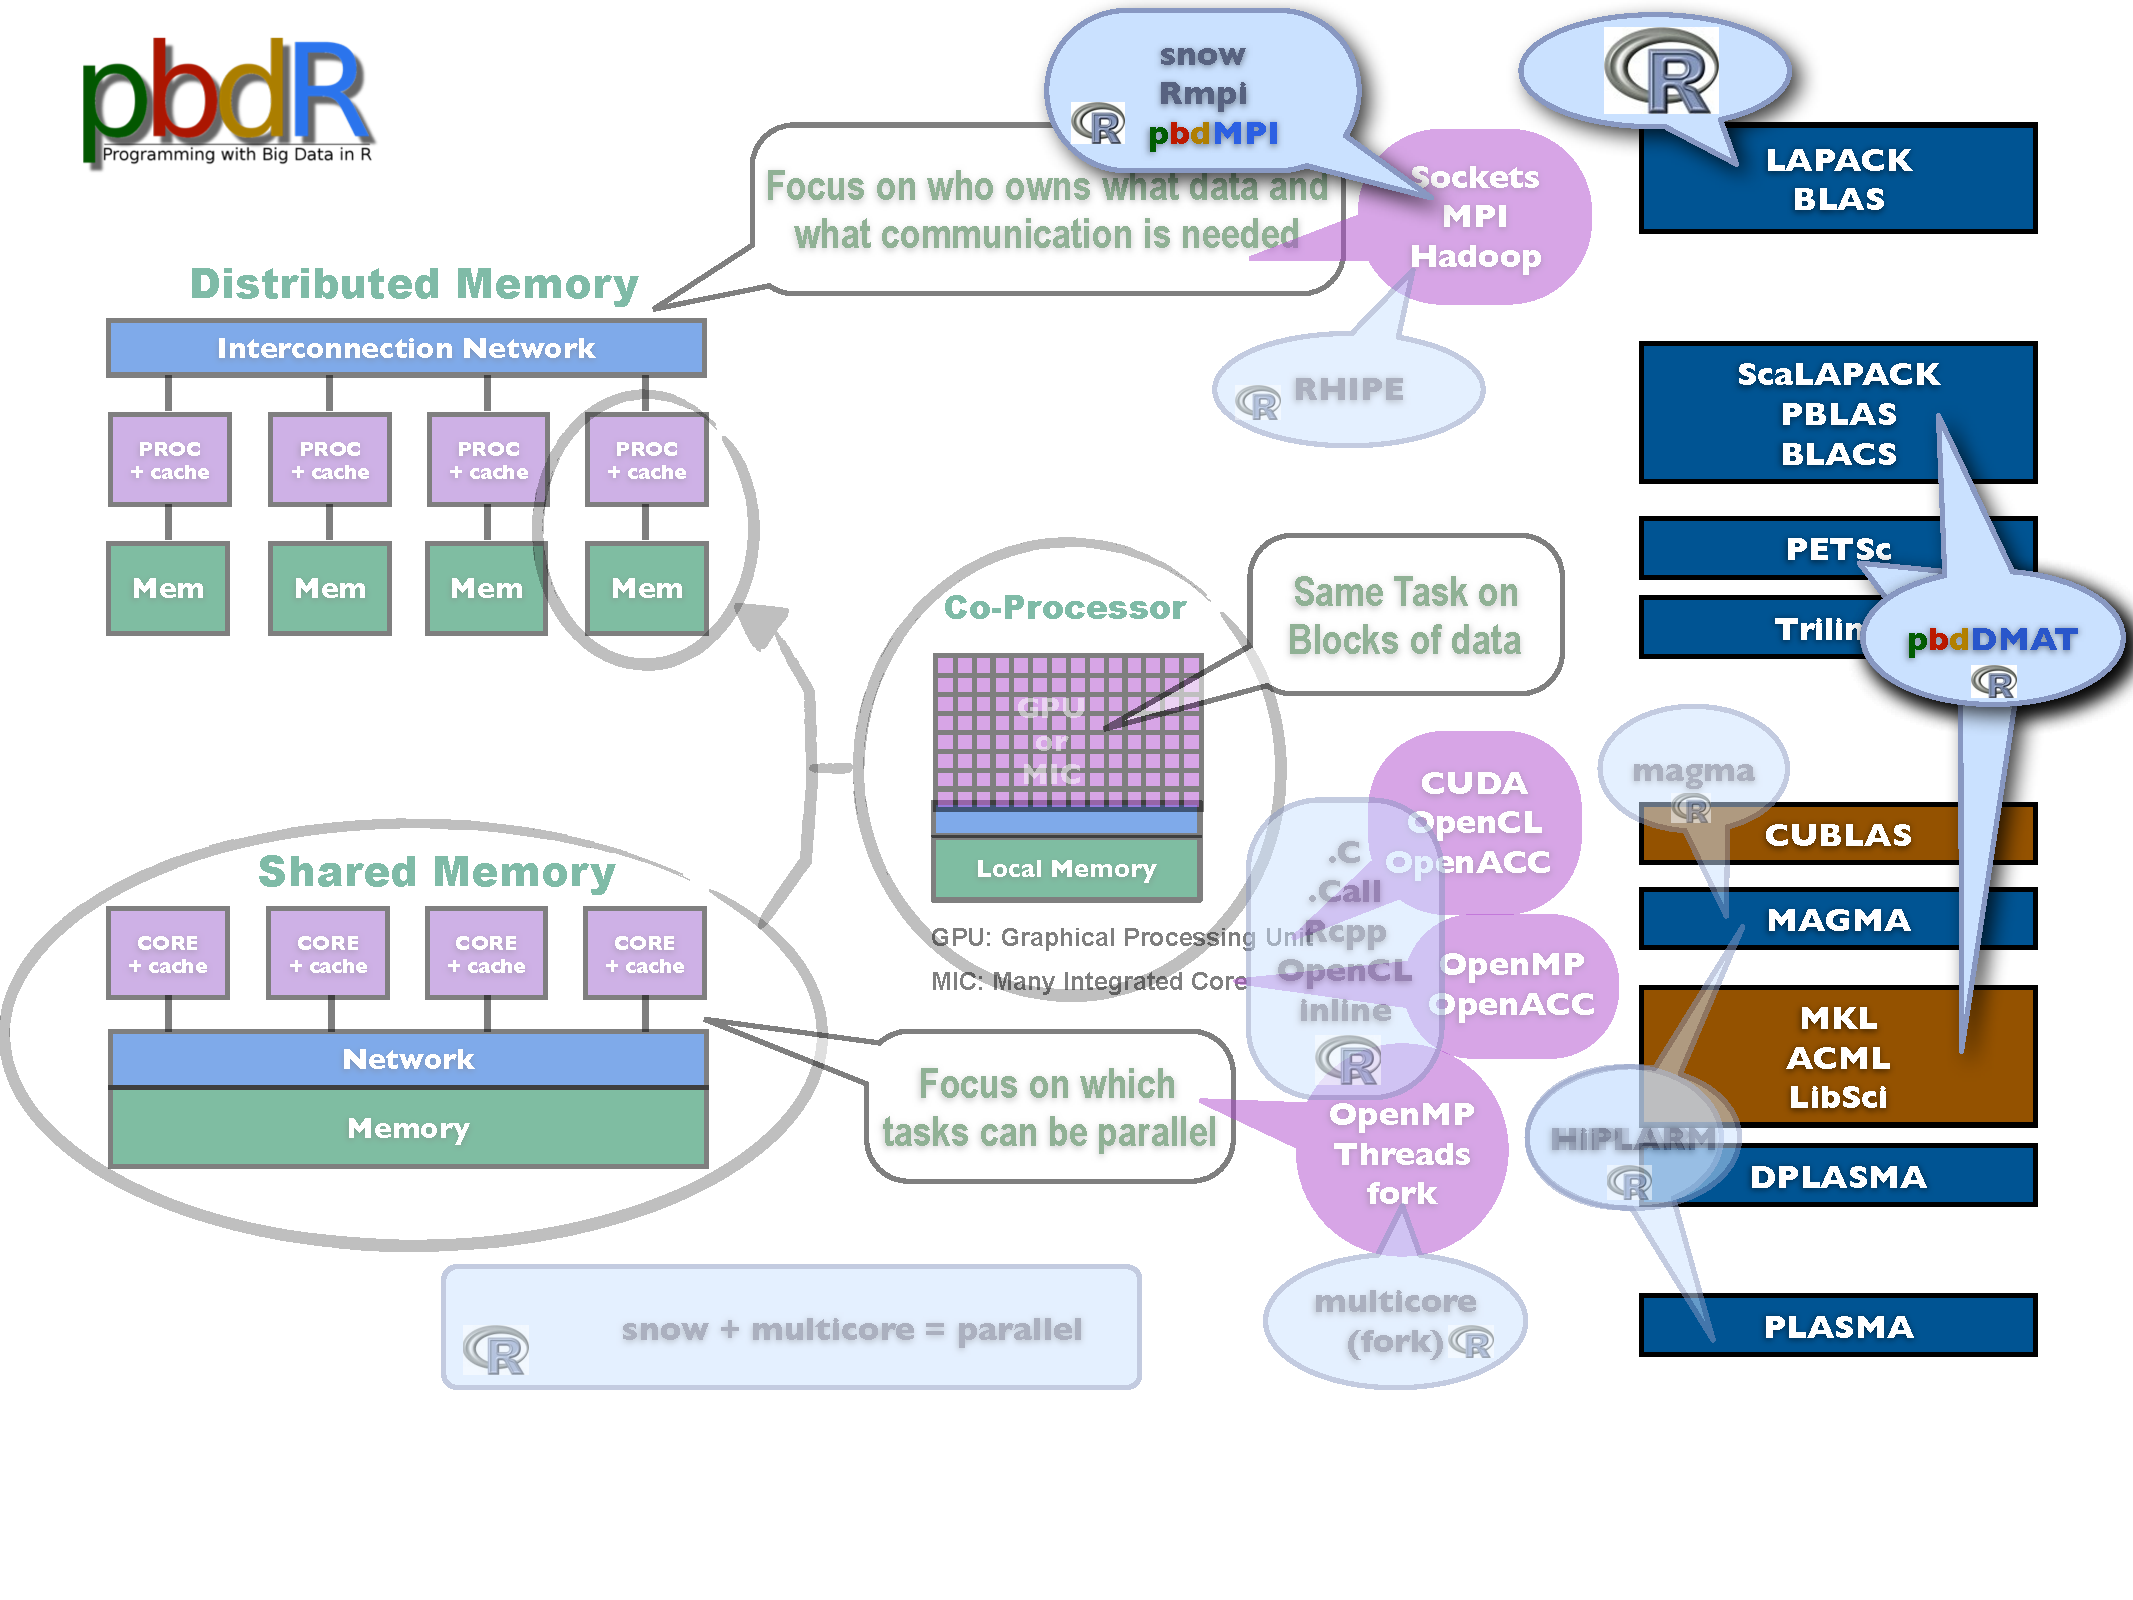
\includegraphics[width=\textwidth,trim=0ex 20ex 0ex 0ex,clip]{../common/pics/hardware/ParallelHardware13.pdf}
  \end{block}
\end{frame}



